\lstdefinestyle{yaml}{
     basicstyle=\color{red}\footnotesize,
     rulecolor=\color{black},
     string=[s]{'}{'},
     stringstyle=\color{red},
     comment=[l]{:},
     commentstyle=\color{black},
     morecomment=[l]{-}
 }
 
\chapter{Proof Of Concept} \label{ch:proofOfConcept}

As the analysis in previous chapters has shown, the Software Defined Vehicle is a pivotal advancement in the evolution of the entire automotive industry toward a safer, more efficient, and more sustainable future. This chapter explores the Proof of Concept (PoC) phase within the context of the thesis, aiming to validate the feasibility and efficacy of implementing SDV technologies. The main objective of this chapter is to translate theoretical concepts into concrete results, demonstrating the practical application of SDV in real-world situations. Through the PoC, we aim to confirm the fundamental principles and features of SDV, including its potential impact on vehicle performance, user experience, and overall safety.
The multifaceted nature of SDV requires a structured approach to its implementation, taking into account factors such as standardized hardware, cloud integration, and over-the-air (OTA) updates. To achieve this, a PoC was designed to address these components individually and holistically, ensuring a seamless integration that aligns with the envisioned paradigm shift in automotive manufacturing. Furthermore, this chapter aims to demonstrate the collaborative efforts with industry-leading technologies and platforms, highlighting the strategic partnerships forged with key players in the automotive and software development sectors. By aligning with renowned entities, the PoC aims to leverage their expertise, technologies, and frameworks, thereby enhancing the robustness and scalability of the SDV ecosystem.
Test and Validation are the concluding phases of this chapter, where the Proof of Concept is subjected to real-world scenarios. A demonstration involving a Raspberry Pi (RPi) serves as a tangible validation of the implemented SDV functionalities. This section serves as the litmus test, affirming the seamless orchestration of SDV within the envisioned architecture.
The exploration of the POC begins by detailing the services and technologies offered by Amazon Web Services (AWS) in the IoT and automotive fields that are essential for project implementation.

\section{Amazon Web Services}

Amazon Web Services (AWS) is a widely adopted cloud solution with over 200 fully featured services available globally across multiple data centers. It is used by millions of customers, from emerging startups to industry giants and government agencies, as the cloud platform of choice to reduce costs, increase agility, and accelerate innovation \cite{EuAmazonWebServices}.

AWS stands out by providing a broad set of services, including infrastructure technologies as well as cutting-edge capabilities such as machine learning, artificial intelligence, data lakes, analytics, and the Internet of Things. This extensive service portfolio facilitates the fast, easy and cost-effective migration of existing applications to the cloud and the creation of diverse digital solutions. AWS provides purpose-built databases for various application types, allowing users to choose the most suitable tool for optimal cost and performance. The depth of AWS services is unmatched, providing customers with a comprehensive toolkit for diverse computing needs.

Beyond its vast offerings, AWS has a large and dynamic global community with millions of active customers and tens of thousands of partners. This inclusive ecosystem spans industries and business sizes, with startups, enterprises, and public sector entities leveraging AWS for a myriad of use cases. The AWS Partner Network (APN) solidifies this network with thousands of system integrators and independent software vendors who adapt their technology to work on AWS.

AWS demonstrates its commitment to innovation through continuous technological advancements. In 2014, AWS launched AWS Lambda, which pioneered serverless computing. This allows developers to run their code without the need to provision or manage servers. Another example is Amazon SageMaker, a fully managed machine learning service that empowers developers to use machine learning without any previous experience.

Rooted in more than 17 years of operational experience, AWS offers unmatched reliability, security, and performance \cite{WhatIsAWS}. Since its establishment in 2006, AWS has become a globally trusted platform, revolutionizing IT infrastructure services by providing a highly reliable, scalable, and cost-effective cloud solution for businesses worldwide in the form of web services with pay-as-you-go pricing \cite{AboutAWS}. One of the key benefits of cloud computing is the ability to replace a company's initial capital expenditures required for infrastructure with low costs that vary as needed and can scale with the business; The characteristics of cloud computing are analyzed in depth below.

\subsection{Cloud Computing}
The National Institute of Standards and Technology (NIST) provides the most comprehensive definition of cloud computing: "Cloud computing is a model for enabling ubiquitous, convenient, on-demand network access to a shared pool of configurable computing resources (e.g., networks, servers, storage, applications, and services) that can be rapidly provisioned and released with minimal management effort or service provider interaction. This cloud model is composed of five essential characteristics, three service models, and four deployment models" \cite{NISTCloudComputing}. This allows for a thorough analysis of the features of cloud computing in relation to AWS services, starting with the five essential characteristics.
\begin{itemize}
    \item \textbf{On-demand self-service:} Consumers can access and allocate computing resources autonomously, such as server time and network storage, without direct involvement with service providers. AWS offers a vast cloud infrastructure with over 200 fully-featured services that consumers can easily access and use from their AWS account.
    \item \textbf{Broad network access:} Resources can be accessed over the network through standard mechanisms, making them usable across various client platforms. In AWS services, this is translated as an on-demand delivery of IT resources over the Internet with pay-as-you-go pricing. 
    \item \textbf{Resource pooling:} Providers pool computing resources in a multi-tenant model, dynamically assigning them based on consumer demand. As said before AWS services are allocable e pagabili in base alle necessità del momento. The customer has limited control over the exact resource location but can specify a higher-level abstraction as country, state, or datacenter. In AWS, clients can select the geographic location of their services through regions. AWS Regions provide access to AWS services that are physically located in a specific geographic area. AWS provides the option to view the availability of a particular service in a specific region, in addition to selecting different regions \cite{AWSRegions}. Resources include storage, processing, memory, and network bandwidth. It also provides services for the Internet of Things, machine learning, data lakes, and analytics.
    \item \textbf{Rapid elasticity:} Resources can be easily adjusted to match fluctuations in demand, either automatically or manually. AWS provides various automated resource allocation systems, including the AWS Cloud Development Kit (AWS CDK) framework, which will be discussed later. The available capabilities are perceived as virtually limitless, and consumers can acquire them in any quantity at any time, always with a pay-per-use system.
    \item \textbf{Measured service:} Cloud systems efficiently manage resources through automated control and optimization, utilizing metering capabilities tailored to specific services such as storage, processing, bandwidth, and user accounts. For instance, AWS has infrastructure worldwide, allowing for easy deployment of applications in multiple physical locations. The proximity to end-users reduces latency and enhances their experience. This feature allows for clear and objective monitoring, control, and reporting of resource usage by both providers and consumers.
\end{itemize}

The three primary types of cloud computing are Infrastructure as a Service (IaaS), Platform as a Service (PaaS), and Software as a Service (SaaS). These options provide different levels of control, flexibility, and management, enabling users to customize services to meet their specific needs \cite{AWSWhatIsCloudComputing}.
\begin{itemize}
    \item \textbf{Infrastructure as a Service (IaaS): } Consumers are able to utilize and deploy fundamental computing resources, including processing, storage, and networks. However, they only have control over operating systems, storage, and applications, as the cloud infrastructure is managed by the provider. Consumer control over some networking components is limited. Infrastructure as a Service (IaaS) provides a high level of flexibility and management control over IT resources. It is similar in practice to existing IT resources that many IT departments and developers are already familiar with. 
    \item \textbf{Platform as a Service (PaaS): } Consumers can deploy their applications on the cloud infrastructure using the programming languages, libraries, services, and tools supported by the provider. The provider manages the underlying cloud infrastructure, including network, servers, operating systems, and storage, while consumers maintain control over their applications and configuration settings. This approach improves efficiency by eliminating the need to manage resource procurement, capacity allocation, software maintenance, patching, or any other tasks involved in running your application. 
    \item \textbf{Software as a Service (SaaS): } Consumers can use the provider's applications on the cloud infrastructure, which are accessible from different client devices through interfaces such as web browsers or programs. However, consumers do not have control over the underlying cloud infrastructure, including the network, servers, operating systems, and storage, except for limited user-specific application configuration settings. With a SaaS offering, users do not need to worry about maintaining the service or managing the underlying infrastructure. The focus should be on how to use the software effectively.
\end{itemize}

The analysis thus far has focused on cloud computing, specifically the essential characteristics that a cloud service must possess to be considered a true cloud service, as well as the service models that can be offered. Now, let's analyze in more detail the part related to cloud computing service deployment models and explore which models are most suitable for which workloads using AWS \cite{AWSPrivatePublicHybrid}. Note that in this case, there are slight differences between the NIST and AWS definitions of the various deployment modes.
\begin{itemize}
    \item \textbf{public cloud: } According to NIST, a public cloud is defined as cloud infrastructure that is publicly accessible and owned, managed, and operated by businesses, academic institutions, government entities, or a combination thereof. In contrast, AWS defines a public cloud as infrastructure and services that are accessible over the public internet and hosted in a specific AWS Region.
    \item \textbf{private cloud: } Both NIST and AWS define private cloud as a cloud infrastructure exclusively provisioned for a single organization, which may own, manage, and operate it independently or in collaboration with a third party. However, there is a difference in the location of the infrastructure. According to NIST, the infrastructure can be located on or off premises, while in AWS documentation, the infrastructure is provisioned on premises using a virtualization layer.
    \item \textbf{hybrid cloud: } The hybrid cloud is a combination of two or more separate cloud infrastructures, private or public, connected by technology to facilitate data and application portability. It allows organizations to leverage the cloud for its efficiency and cost savings while also maintaining on-site security, privacy, and control.
\end{itemize}

Exploring the many benefits of cloud computing, the focus now shifts to a comprehensive analysis of the main value patterns of cloud computing, with some charts and graphs to help clarify the outlook.

When analyzing the resources required by a business, it becomes clear that satisfying demand through local services and resources often requires a monetary expenditure of resources that exceeds actual demand. This results in a wastage of resources that could be allocated more efficiently. On the other hand, the opposite situation may also occur, as shown in \ref{tab:OperatingExpenditureValueModel} within the same domain, where there is a higher demand than the available resources. The adoption of cloud computing transforms this paradigm. With AWS, you can pay only for the computing resources you consume and exclusively for the amount you utilize. This approach enables more cost-effective and streamlined resource utilization.
\begin{table}[h]
    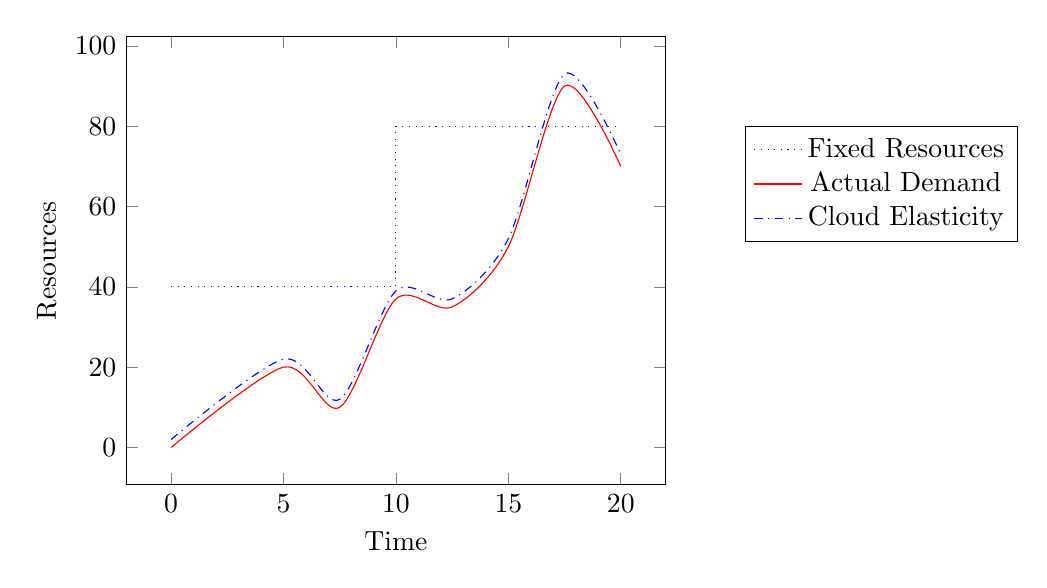
\begin{tikzpicture}
        \begin{axis}[xlabel={Time}, ylabel={Resources}, legend style={at={(1.4,0.8)},anchor=north},]
            % Fixed Resources line
            \addplot[blue,mark=none, dotted] coordinates {(0,40) (10,40) (10,80) (20,80)};
            \addlegendentry{Fixed Resources}
        
            % Actual Demand line
            \addplot[red,mark=none, smooth] coordinates {(0,0) (5,20) (7.5,10) (10,37) (12.5,35) (15, 50) (17.5, 90) (20, 70)};
            \addlegendentry{Actual Demand}
        
            % Cloud Elasticity line
            \addplot[blue,mark=none, smooth, dash dot] coordinates {(0,2) (5,22) (7.5,12) (10,39) (12.5,37) (15, 52) (17.5, 93) (20, 73)};
            \addlegendentry{Cloud Elasticity}
        \end{axis}
    \end{tikzpicture}
    \caption{Operating expenditure value model \cite{CloudComputing}}
    \label{tab:OperatingExpenditureValueModel}
\end{table}

Cloud computing also reduces costs by aggregating resources needed by different companies in a transparent way to consumers. In addition to shortening the time to market and increasing earnings, cloud computing allows for access to resources anytime and anywhere, optimizing resource management with lower latency and a better experience as it is shown in ref{LocationFlexibilityValueModel}.
\begin{table}[h]
    \begin{tikzpicture}
        \begin{axis}[xlabel={Location}, ylabel={Availability}, ytick={10,80}, yticklabels={Low, High}, legend style={at={(1.4,0.8)},anchor=north},]
            % Traditional Computing line
            \addplot[blue,mark=none,] coordinates {(0,20) (5,30) (7.5,35) (10,40) (12.5,35) (15, 50) (17.5, 60) (20, 55)};
            \addlegendentry{Traditional Computing}
        
            % Cloud Computing line
            \addplot[blue,mark=none, smooth, dotted] coordinates {(0,80) (5,80) (10,80) (15, 80) (20, 80)};
            \addlegendentry{Cloud Computing}
        \end{axis}
    \end{tikzpicture}
    \caption{Location flexibility value model \cite{CloudComputing}}
    \label{tab:LocationFlexibilityValueModel}
\end{table}

UTILIZZARE IL SEGUETE TESTO COME DISCORSO CONCLUSIVO SUL CLOUD COMPUTING
Cloud computing is the on-demand delivery of IT resources over the Internet with pay-as-you-go pricing. Instead of buying, owning, and maintaining physical data centers and servers, you can access technology services, such as computing power, storage, and databases, on an as-needed basis from a cloud provider like Amazon Web Services (AWS). Organizations of every type, size, and industry are using the cloud for a wide variety of use cases, such as data backup, disaster recovery, email, virtual desktops, software development and testing, big data analytics, and customer-facing web applications. For example, healthcare companies are using the cloud to develop more personalized treatments for patients. Financial services companies are using the cloud to power real-time fraud detection and prevention. And video game makers are using the cloud to deliver online games to millions of players around the world. 
The cloud gives you easy access to a broad range of technologies so that you can innovate faster and build nearly anything that you can imagine. You can quickly spin up resources as you need them-from infrastructure services, such as compute, storage, and databases, to Internet of Things, machine learning, data lakes and analytics, and much more. You can deploy technology services in a matter of minutes, and get from idea to implementation several orders of magnitude faster than before. This gives you the freedom to experiment, test new ideas to differentiate customer experiences, and transform your business.
With cloud computing, you don't have to over-provision resources up front to handle peak levels of business activity in the future. Instead, you provision the amount of resources that you actually need. You can scale these resources up or down to instantly grow and shrink capacity as your business needs change.
The cloud allows you to trade fixed expenses (such as data centers and physical servers) for variable expenses, and only pay for IT as you consume it. Plus, the variable expenses are much lower than what you would pay to do it yourself because of the economies of scale. 
With the cloud, you can expand to new geographic regions and deploy globally in minutes.


%https://ieeexplore.ieee.org/document/8114187?denied=
%https://ieeexplore.ieee.org/document/9044834



\subsection{Security}
One of the pillars of AWS is the security of its systems and services; data la natura della tesi analizziamo più nel dettaglio questa caratteristica.

AWS is architected to be the most flexible and secure cloud computing environment available today. Our core infrastructure is built to satisfy the security requirements for the military, global banks, and other high-sensitivity organizations. This is backed by a deep set of cloud security tools, with over 300 security, compliance, and governance services and features, as well as support for 143 security standards and compliance certifications.

AWS infrastructure has been architected to be one of the most flexible and secure cloud computing environments available today. It is designed to provide an extremely scalable, highly reliable platform that enables customers to deploy applications and data quickly and securely. This infrastructure is built and managed not only according to security best practices and standards, but also with the unique needs of the cloud in mind. AWS uses redundant and layered controls, continuous validation and testing, and a substantial amount of automation to ensure that the underlying infrastructure is monitored and protected 24x7. IT Security is often not the core business of our customers. IT departments operate on limited budgets and do a good job of securing their data centers and software given limited resources. In the case of AWS, security is foundational to our core business and so significant resources are applied to ensuring the security of the cloud and helping our customers ensure security in the cloud, as described further below \cite{AWSCloudComputing}. 

Strong security at the core of an organization enables digital transformation and innovation. AWS helps organizations to develop and evolve security, identity, and compliance into key business enablers. At AWS, security is our top priority. AWS is architected to be the most secure global cloud infrastructure on which to build, migrate, and manage applications and workloads. This is backed by our deep set of 300+ cloud security tools and the trust of our millions of customers, including the most security sensitive organizations like government, healthcare, and financial services.

We innovate on behalf of our customers so they can move quickly, securely, and with confidence to enable their business. With AWS cloud infrastructure, and our broad set of security services, and partners, our customers integrate powerful security technology and control to enable their business to innovate securely. Build, run, and scale your applications on infrastructure architected to be the most secure cloud computing environment available today. As organizations migrate and build on cloud, they need assurance that they have a secure foundation. AWS has the most proven operational experience of any cloud provider. Our cloud infrastructure is highly trusted and secure-by-design, giving customers the confidence to accelerate innovation. Move fast and stay secure by confidently integrating and automating security into every part of your organization. Building securely should be the path of least resistance - with no tradeoff between security with speed. With security automation, teams spend their limited time on the highest value tasks, reduce human error, and scale security best practices across the organization. Innovate with a wide portfolio of security services and partner solutions to help achieve end-to-end security for your organization. Organizations require powerful capabilities, designed and built by experts, which encode years of experience, knowledge and best practices, all available at their fingertips. They don't want to navigate this changing threat and compliance landscape alone \cite{AWSSecurity}.

The AWS global infrastructure is designed and managed according to security best practices as well as a variety of security compliance standards. With AWS, you can be assured that you are building web architectures on top of some of the most secure computing infrastructure in the world. The IT infrastructure that AWS provides to you is designed and managed in alignment with security best practices and a variety of IT security standards including the following that life science customers may find most relevant \cite{AWSCertificationsAndAttestations}: 
\begin{itemize}
    \item SOC 1, 2, 3:  AWS System and Organization Controls (SOC) Reports are independent third-party examination reports that demonstrate how AWS achieves key compliance controls and objectives. The purpose of these reports is to help you and your auditors understand the AWS controls established to support operations and compliance. The SOC 1 reports are designed to focus on controls at a service organization that are likely to be relevant to an audit of a user entity's financial statements. The AWS SOC 1 report is designed to cover specific key controls likely to be required during a financial audit, as well as covering a broad range of IT general controls to accommodate a wide range of usage and audit scenarios. The AWS SOC1 control objectives include security organization, employee user access, logical security, secure data handling, physical security and environmental protection, change management, data integrity, availability and redundancy and incident handling. The SOC 2 report is an attestation report that expands the evaluation of controls to the criteria set forth by the American Institute of Certified Public Accountants (AICPA) Trust Services Principles. These principles define leading practice controls relevant to security, availability, processing integrity, confidentiality, and privacy applicable to service organizations such as AWS. The AWS SOC 2 is an evaluation of the design and operating effectiveness of controls that meet the criteria for the security and availability principles set forth in the AICPA's Trust Services Principles criteria. This report provides additional transparency into AWS security and availability based on a pre-defined industry standard of leading practices and further demonstrates the commitment of AWS to protecting customer data. The SOC2 report information includes outlining AWS controls, a description of AWS Services relevant to security, availability and confidentiality as well as test results against controls. You will likely find the SOC 2 report to be the most detailed and relevant SOC report as it relates to GxP compliance. AWS publishes a Service Organization Controls 3 (SOC 3) report. The SOC 3 report is a publicly-available summary of the AWS SOC 2 report. The report includes the external auditor's assessment of the operation of controls (based on the AICPA's Security Trust Principles included in the SOC 2 report), the assertion from AWS management regarding the effectiveness of controls, and an overview of AWS Infrastructure and Services. 
    \item FedRAMP: The Federal Risk and Authorization Management Program (FedRAMP) is a US government-wide program that delivers a standard approach to the security assessment, authorization, and continuous monitoring for cloud products and services. FedRAMP uses the NIST Special Publication 800 series and requires cloud service providers to receive an independent security assessment conducted by a third-party assessment organization (3PAO) to ensure that authorizations are compliant with the Federal Information Security Management Act (FISMA).
    \item ISO 9001: ISO 9001:2015 outlines a process-oriented approach to documenting and reviewing the structure, responsibilities, and procedures required to achieve effective quality management within an organization. Specific sections of the standard contain information on topics such as: Requirements for a quality management system (QMS), including documentation of a quality manual, document control, and determining process interactions; Responsibilities of management; Management of resources, including human resources and an organization's work environment; Service development, including the steps from design to delivery; Customer satisfaction; Measurement, analysis, and improvement of the QMS through activities like internal audits and corrective and preventive actions. The AWS ISO 9001:2015 certification directly supports customers who develop, migrate and operate their quality-controlled IT systems in the AWS cloud. You can leverage AWS compliance reports as evidence for your own ISO 9001:2015 programs and industry-specific quality programs, such as GxP in life sciences and ISO 131485 in medical devices. 
    \item ISO/IEC 27001: ISO/IEC 27001:2013 is a widely-adopted global security standard that sets out requirements and best practices for a systematic approach to managing company and customer information that's based on periodic risk assessments appropriate to ever-changing threat scenarios. In order to achieve the certification, a company must show it has a systematic and ongoing approach to managing information security risks that affect the confidentiality, integrity, and availability of company and customer information. This widely-recognized international security standard specifies that AWS do the following: We systematically evaluate AWS information security risks, taking into account the impact of threats and vulnerabilities; We design and implement a comprehensive suite of information security controls and other forms of risk management to address customer and architecture security risks; We have an overarching management process to ensure that the information security controls meet our needs on an ongoing basis. AWS has achieved ISO 27001 certification of the Information Security Management System (ISMS) covering AWS infrastructure, data centers, and services.
    \item ISO/IEC 27017: ISO/IEC 27017:2015 provides guidance on the information security aspects of cloud computing, recommending the implementation of cloud-specific information security controls that supplement the guidance of the ISO/IEC 27002 and ISO/IEC 27001 standards. This code of practice provides additional information security controls implementation guidance specific to cloud service providers. The AWS attestation to the ISO/IEC 27017:2015 standard not only demonstrates an ongoing commitment to align with globally-recognized best practices, but also verifies that AWS has a system of highly precise controls in place that are specific to cloud services.
    \item ISO/IEC 27018: ISO 27018 is the first International code of practice that focuses on protection of personal data in the cloud. It is based on ISO information security standard 27002 and provides implementation guidance on ISO 27002 controls applicable to public cloud Personally Identifiable Information (PII). It also provides a set of additional controls and associated guidance intended to address public cloud PII protection requirements not addressed by the existing ISO 27002 control set. AWS has achieved ISO 27018 certification, an internationally recognized code of practice, which demonstrates the commitment of AWS to the privacy and protection of your content.
    \item HITRUST: The Health Information Trust Alliance Common Security Framework (HITRUST CSF) leverages nationally and internationally accepted standards and regulations such as GDPR, ISO, NIST, PCI, and HIPAA to create a comprehensive set of baseline security and privacy controls. HITRUST has developed the HITRUST CSF Assurance Program, which incorporates the common requirements, methodology, and tools that enable an organization and its business partners to take a consistent and incremental approach to managing compliance. Further, it allows business partners and vendors to assess and report against multiple sets of requirements. Certain AWS services have been assessed under the HITRUST CSF Assurance Program by an approved HITRUST CSF Assessor as meeting the HITRUST CSF Certification Criteria. The certification is valid for two years, describes the AWS services that have been validated, and can be publiccaly accessed. You may look to leverage the AWS HITRUST CSF certification of AWS services to support your own HITRUST CSF certification, in complement to your GxP compliance programs.
    \item CSA Security, Trust and Assurance Registry (STAR): In 2011, the Cloud Security Alliance (CSA) launched STAR, an initiative to encourage transparency of security practices within cloud providers. The CSA Security, Trust and Assurance Registry (STAR) is a free, publicly accessible registry that documents the security controls provided by various cloud computing offerings, thereby helping users assess the security of cloud providers they currently use or are considering. AWS participates in the voluntary CSA Security, Trust and Assurance Registry (STAR) Self-Assessment to document AWS compliance with CSA-published best practices. AWS publishes the completed CSA Consensus Assessments Initiative Questionnaire (CAIQ) on the AWS website.
\end{itemize}

GxP is an acronym that refers to the regulations and guidelines applicable to life sciences organizations that make food and medical products such as drugs, medical devices, and medical software applications. The overall intent of GxP requirements is to ensure that food and medical products are safe for consumers and to ensure the integrity of data used to make product-related safety decisions. The term GxP encompasses a broad range of compliance-related activities such as Good Laboratory Practices (GLP), Good Clinical Practices (GCP), Good Manufacturing Practices (GMP), and others, each of which has product-specific requirements that life sciences organizations must implement based on the 1) type of products they make and 2) country in which their products are sold. When life sciences organizations use computerized systems to perform certain GxP activities, they must ensure that the computerized GxP system is developed, validated, and operated appropriately for the intended use of the system. \cite{GxPCompliance}
\subsection{Used services}

\section{Design}
\subsection{Architecture}

\section{Implementation}
\subsection{Code}
\subsection{Tools}

\section{Test and Validation}
\subsection{RPi demo}